\section{Results}
\label{sec:results}

\subsection{Main Accuracy Results}

\begin{table}[t]
    \centering
    \resizebox{\textwidth}{!}{%
    \begin{tabular}{@{}llcccc@{}}
        \toprule
        \textbf{Pair labels} & \textbf{Method} & \textbf{IID acc. (\%)} & \textbf{OOD acc. (\%)} & \textbf{OOD 95\% CI (\%)} & \textbf{Digit acc. (\%)} \\
        \midrule
        1,000 & \directsum & 14.3 & {\bf 1.4} & [1.2, 1.6] & -- \\
        1,000 & \symbolicsum & 17.3 & 0.0 & [0.0, 0.0] & 29.4 \\
        1,000 & \anchorsymbolic & {\bf 19.9} & 0.0 & [0.0, 0.0] & {\bf 34.1} \\
        1,000 & \anchorposterior & 18.9 & 0.0 & [0.0, 0.0] & 33.4 \\
        \midrule
        5,000 & \directsum & 31.8 & 0.3 & [0.2, 0.4] & -- \\
        5,000 & \symbolicsum & {\bf 90.0} & {\bf 82.5} & [81.8, 83.2] & {\bf 93.8} \\
        5,000 & \anchorsymbolic & 87.7 & 73.2 & [72.4, 74.0] & 91.8 \\
        5,000 & \anchorposterior & 88.0 & 74.1 & [73.3, 74.8] & 92.0 \\
        \bottomrule
    \end{tabular}
    }
    \caption{Main AddMNIST results across budgets. Higher is better for all accuracy columns. Best result within each pair-label budget and metric is in {\bf bold}. OOD confidence intervals are bootstrap 95\% intervals over 12,000 predictions per method-budget condition.}
    \label{tab:main_results}
\end{table}


\Figref{fig:accuracy_budget} and \tabref{tab:main_results} show the main result. At 1,000 pair labels, none of the symbolic models learns a reliable enough digit grounding to solve the high-plus-high split. \directsum obtains 1.4\% OOD accuracy, while all symbolic variants obtain 0.0\%. This low-budget result is important: symbolic structure does not remove the need to learn usable predicates.

At 5,000 pair labels, the behavior changes sharply. \symbolicsum reaches 90.0\% IID accuracy and 82.5\% OOD high-plus-high accuracy. \directsum improves to 31.8\% IID accuracy but remains at 0.3\% OOD accuracy. The absolute OOD gap between \symbolicsum and \directsum is 82.2 percentage points. The anchor variants also strongly beat the direct baseline, reaching 73.2\% and 74.1\% OOD accuracy, but they do not exceed the plain symbolic likelihood.

\begin{figure}[t]
    \centering
    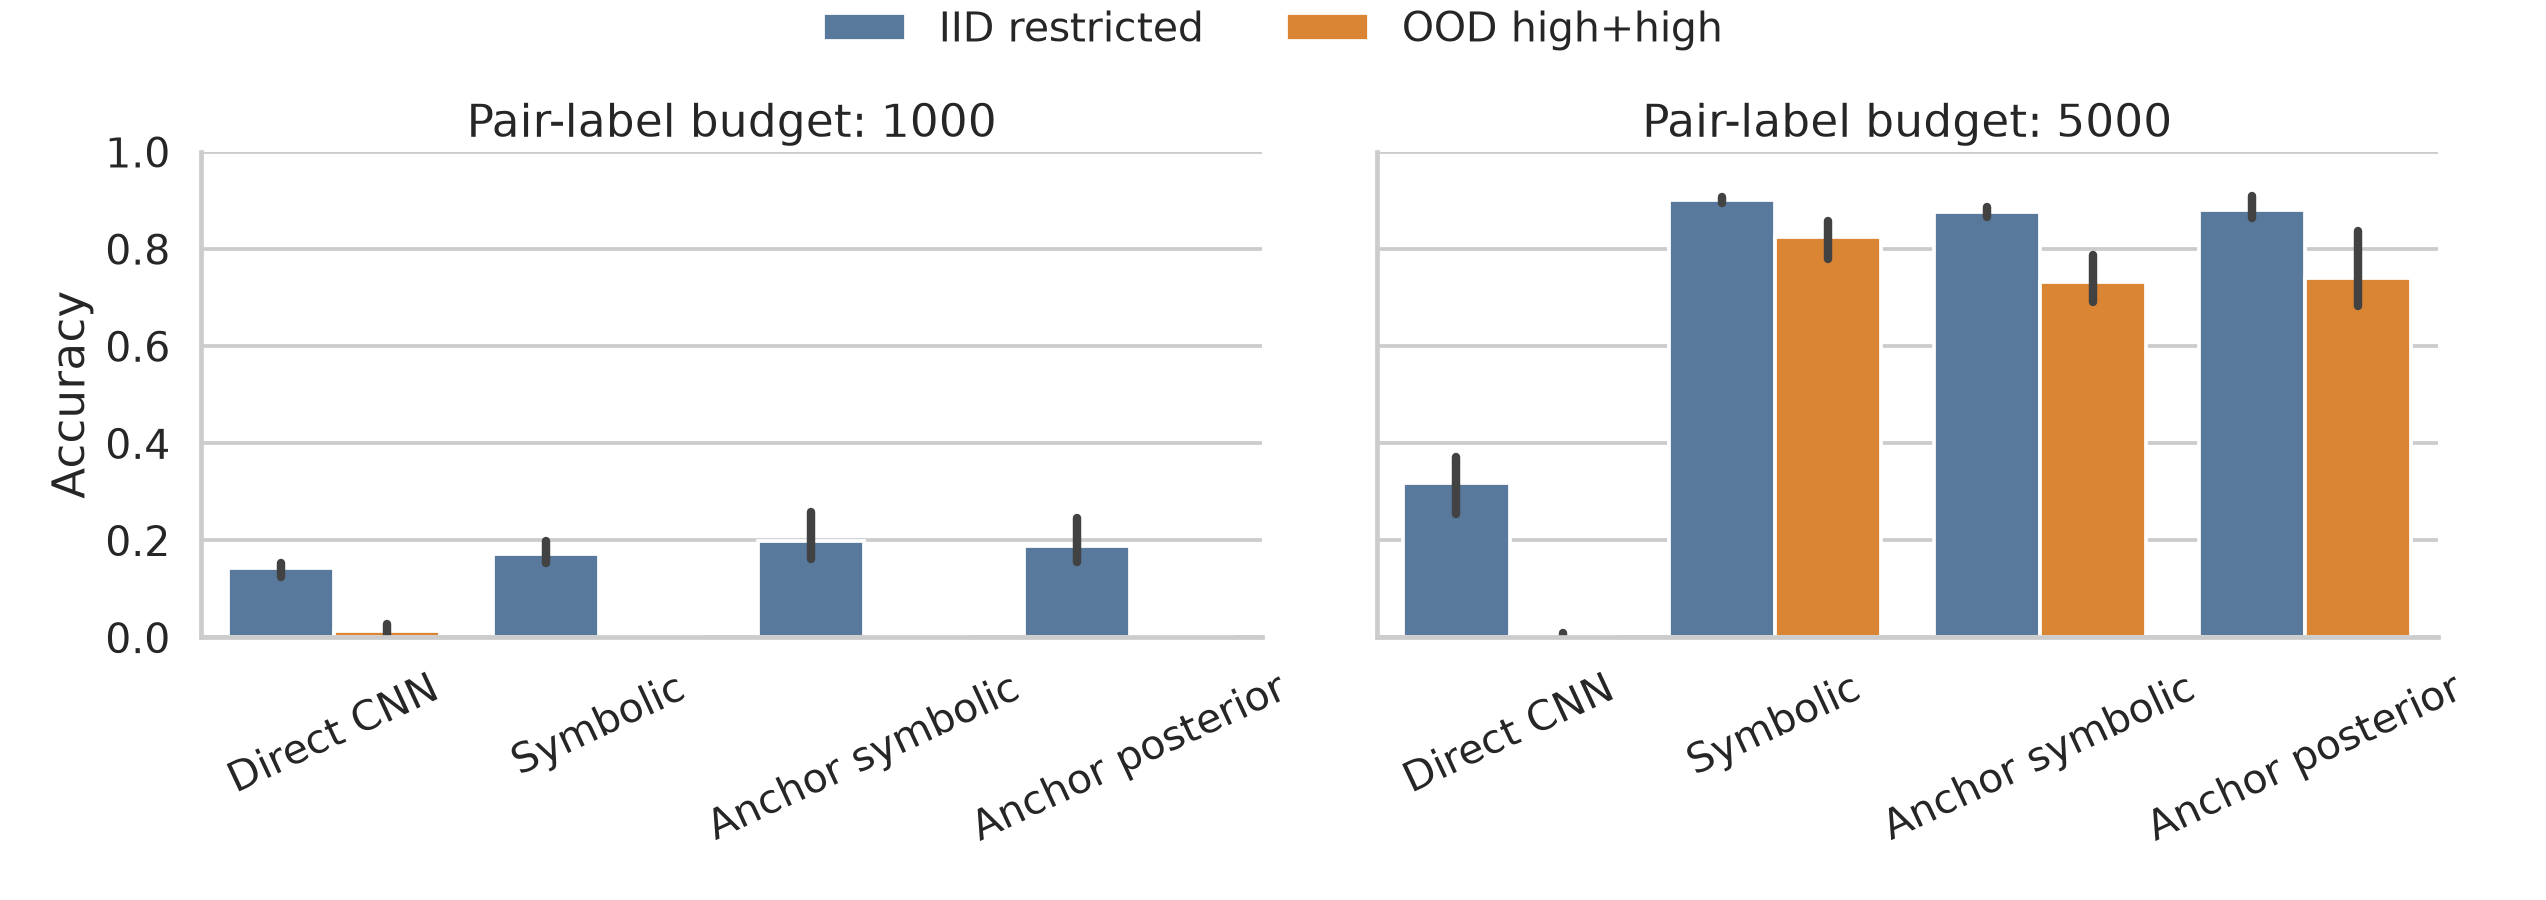
\includegraphics[width=0.95\linewidth]{figures/accuracy_by_method_budget.png}
    \caption{Accuracy by method and pair-label budget. The 5,000-label setting separates the direct classifier from the neural-symbolic models: exact symbolic marginalization enables high OOD accuracy once digit predicates are grounded.}
    \label{fig:accuracy_budget}
\end{figure}

\subsection{Extrapolation to Unseen Sum Labels}

\begin{table}[t]
    \centering
    \resizebox{\textwidth}{!}{%
    \begin{tabular}{@{}lcccc@{}}
        \toprule
        \textbf{Method} & \textbf{Seen OOD sums 10--13 (\%)} & \textbf{Examples} & \textbf{Unseen sums 14--18 (\%)} & \textbf{Examples} \\
        \midrule
        \directsum & 0.9 & 4,432 & 0.0 & 7,568 \\
        \symbolicsum & {\bf 85.7} & 4,432 & {\bf 80.6} & 7,568 \\
        \anchorsymbolic & 79.2 & 4,432 & 69.7 & 7,568 \\
        \anchorposterior & 80.6 & 4,432 & 70.3 & 7,568 \\
        \bottomrule
    \end{tabular}
    }
    \caption{OOD high-plus-high accuracy at the 5,000-label budget, split by whether the target sum label appeared in training. Sums 14--18 never appear as supervised training labels because training excludes high-plus-high pairs.}
    \label{tab:ood_regions}
\end{table}


The main OOD split contains both seen and unseen sum labels. Sums 10--13 can occur during restricted training through low-plus-high pairs, while sums 14--18 cannot occur because both digits must be high. \Tabref{tab:ood_regions} separates these regions for the 5,000-label budget. \symbolicsum reaches 85.7\% accuracy on seen OOD sums and 80.6\% accuracy on unseen sums 14--18. \directsum reaches 0.9\% on seen OOD sums and 0.0\% on unseen sums. The direct model has output logits for the unseen labels, but the training objective never rewards those labels, so it has no effective route to the held-out sums.

\begin{figure}[t]
    \centering
    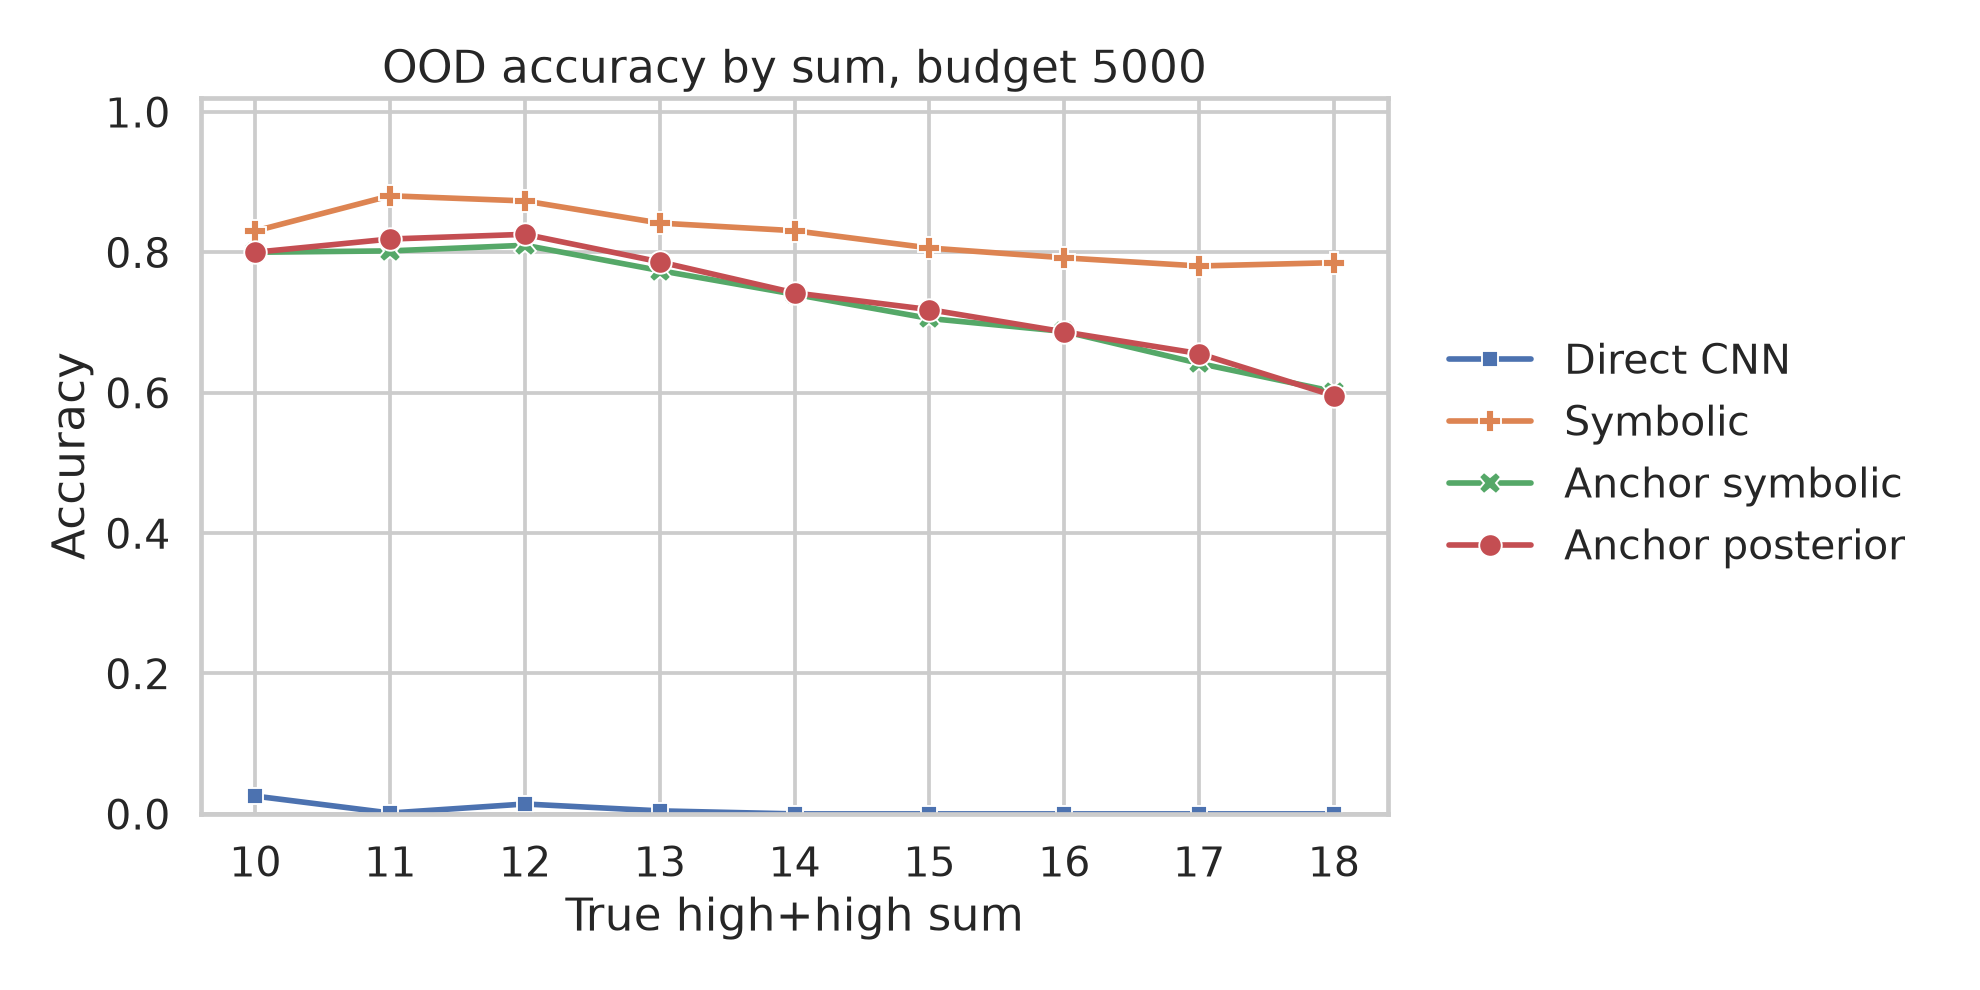
\includegraphics[width=0.95\linewidth]{figures/ood_accuracy_by_sum.png}
    \caption{OOD accuracy by true sum. The symbolic models recover high-plus-high sums across the OOD range at the 5,000-label budget, including sums 14--18 that never appear as training labels.}
    \label{fig:ood_by_sum}
\end{figure}

\subsection{Digit Grounding}

\begin{table}[t]
    \centering
    \begin{tabular}{@{}lcc@{}}
        \toprule
        \textbf{Method} & \textbf{1,000 labels digit acc. (\%)} & \textbf{5,000 labels digit acc. (\%)} \\
        \midrule
        \symbolicsum & 29.4 {\scriptsize $\pm$ 4.8} & {\bf 93.8} {\scriptsize $\pm$ 0.8} \\
        \anchorsymbolic & {\bf 34.1} {\scriptsize $\pm$ 6.1} & 91.8 {\scriptsize $\pm$ 1.1} \\
        \anchorposterior & 33.4 {\scriptsize $\pm$ 5.9} & 92.0 {\scriptsize $\pm$ 2.2} \\
        \bottomrule
    \end{tabular}
    \caption{Digit grounding accuracy for symbolic models on the MNIST test split. Values report mean and standard deviation over three seeds.}
    \label{tab:digit_grounding}
\end{table}


The OOD gains coincide with strong digit grounding. At 1,000 pair labels, symbolic models reach only 29.4--34.1\% digit accuracy, and OOD accuracy remains at zero. At 5,000 pair labels, digit accuracy rises above 91\% for all symbolic variants. The strongest OOD model, \symbolicsum, also has the strongest digit grounding at 93.8\% mean digit accuracy. This supports the intended interpretation: the model is not merely fitting aggregate sum labels; it learns reusable digit predicates that the addition table can compose.

\begin{figure}[t]
    \centering
    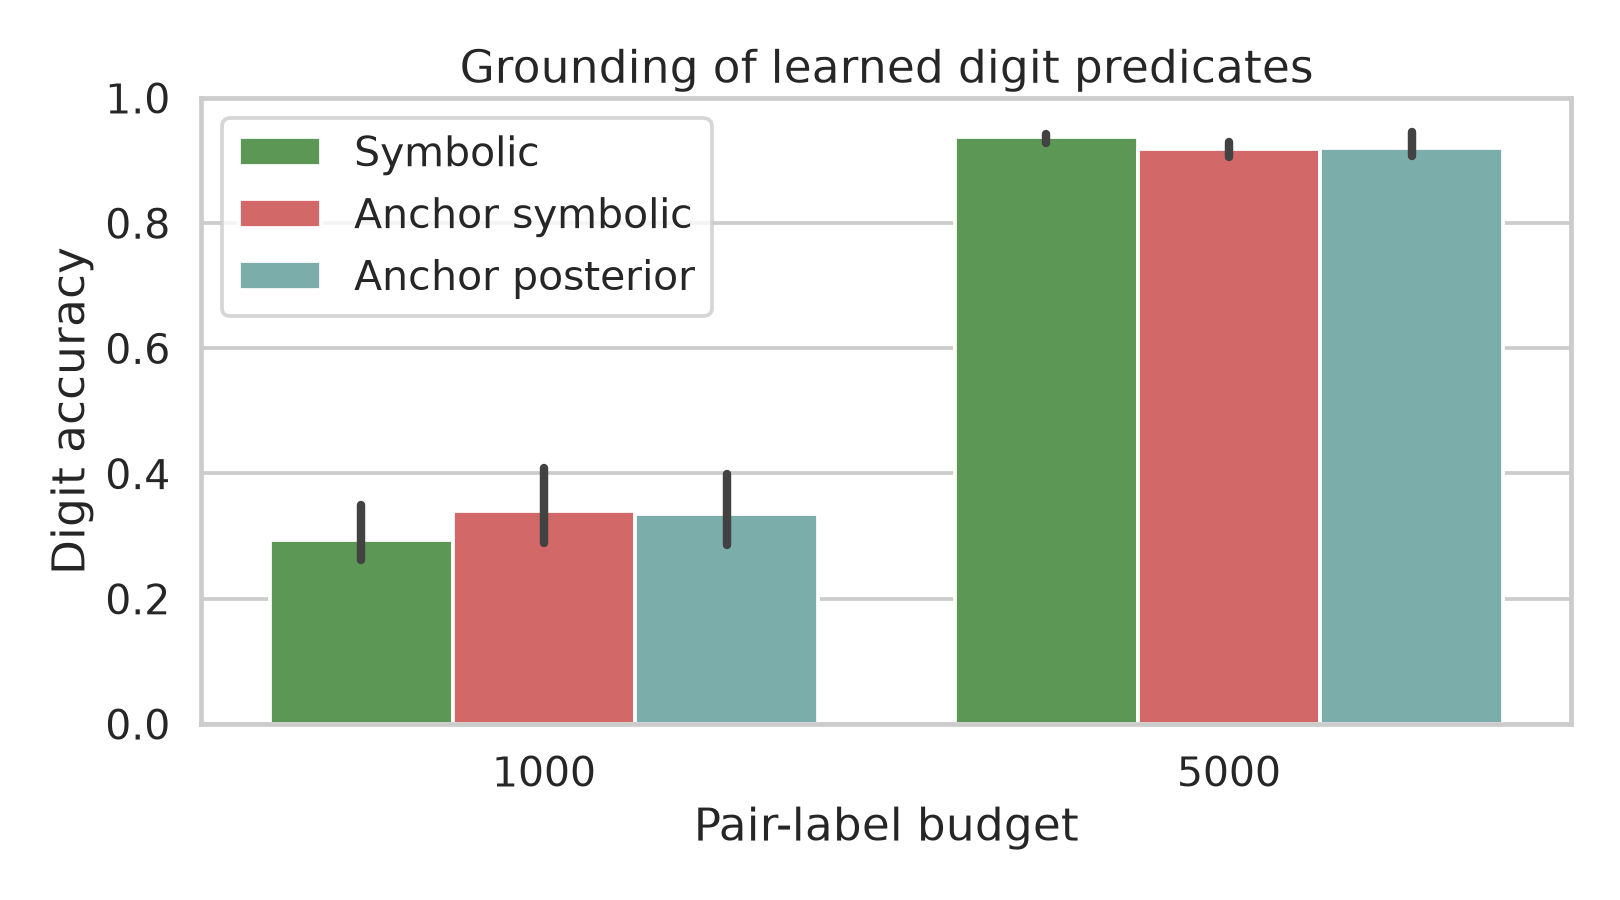
\includegraphics[width=0.78\linewidth]{figures/digit_grounding.png}
    \caption{Digit grounding accuracy for symbolic models. OOD sum generalization appears only when the learned digit predicates become accurate enough to support symbolic composition.}
    \label{fig:digit_grounding}
\end{figure}

\subsection{Statistical Comparisons}

\begin{table}[t]
    \centering
    \resizebox{\textwidth}{!}{%
    \begin{tabular}{@{}lcccccc@{}}
        \toprule
        \textbf{Method A} & \textbf{Method B} & \textbf{Mean A (\%)} & \textbf{Mean B (\%)} & \textbf{Diff. (\%)} & \textbf{Cohen's $d_z$} & \textbf{$p$-value} \\
        \midrule
        \anchorposterior & \directsum & 74.1 & 0.3 & 73.8 & 9.33 & 0.0038 \\
        \anchorsymbolic & \directsum & 73.2 & 0.3 & 72.9 & 16.67 & 0.0012 \\
        \symbolicsum & \directsum & {\bf 82.5} & 0.3 & {\bf 82.2} & {\bf 20.75} & {\bf 0.0008} \\
        \bottomrule
    \end{tabular}
    }
    \caption{Paired seed-level tests for OOD high-plus-high accuracy at the 5,000-label budget. Tests use three matched seeds and should be read as descriptive because the seed count is small.}
    \label{tab:stats}
\end{table}


\Tabref{tab:stats} reports paired seed-level tests for the 5,000-label OOD setting. The symbolic likelihood model improves over \directsum by 82.2 percentage points, with Cohen's $d_z=20.75$ and $p=0.0008$ across three matched seeds. The anchor variants also show large gains over \directsum. Because there are only three seeds, we treat the $p$-values as descriptive rather than definitive. The bootstrap intervals over per-example predictions tell the same story: \symbolicsum has an OOD interval of [81.8, 83.2]\%, while \directsum has [0.2, 0.4]\%.

\subsection{Ablation Summary}

The planned anchor-posterior modification is useful as an ablation but not as the best-performing method. At 5,000 labels, \anchorposterior reaches 74.1\% OOD accuracy, slightly above \anchorsymbolic at 73.2\%, but both trail \symbolicsum at 82.5\%. The anchor and entropy terms may over-weight early latent assignments or interfere with the weak pair-label signal. The result is a negative finding for the proposed modification and a positive finding for the simpler symbolic likelihood.
